\par\SourceLeaf{410}\Needspace{10\baselineskip}\begin{center}[3.]\end{center}
\noindent\hspace*{1.2em}Hauptmomente des Beweises der vorstehenden Lehrsätze sind folgende.

Es sei $r$ die Länge einer vom Punkt $A$ auslaufenden kürzesten Linie auf der krummen Fläche, $\theta$ der Winkel, den sie mit einer ähnlichen festen Linie macht, $\BareRoot{\frac1f}$ Halbmesser der Kugel, die dieselbe Krümmung hat, wie die krumme Fläche am Endpunkte von $r$, $\rho d\theta$ das Linearelement zwischen zwei Punkten, denen $r,\theta$ und $r,\theta+d\theta$ zugehören. Es werden demnach sowohl $f$ als $\rho$ Functionen von $r$ und $\theta$ sein und man hat
\[
\frac{\partial\partial\rho}{\partial r^2}=-f\rho.
\]
\indent Es sei $dt$ ein Element einer zweiten kürzesten Linie und $\zeta$ sein Winkel mit dem zugehörigen $r$. Man hat dann
\[
dr=dt.\cos\zeta,\quad\rho d\theta=dt.\sin\zeta,\quad d\zeta=-\frac{\partial\rho}{\partial r}.d\theta.
\]
\noindent Setzt man
\[
f=F+F'r+F''rr+.\, .\, .,
\]
\noindent so wird
\[
\begin{aligned}
\rho={}&r+*-\tfrac16Fr^3-\tfrac1{12}F'r^4-(\tfrac1{20}F''-\tfrac1{120}FF)r^5\\
&-(\tfrac1{30}F'''-\tfrac1{120}FF')r^6+.\, .\, .\\
\rho={}&r+*-\tfrac1{12}(F+f)r^3+*+(\tfrac1{30}F''+\tfrac1{120}FF)r^5\\
&+(\tfrac1{20}F'''+\tfrac1{120}FF')r^6+.\, .\, .
\end{aligned}
\]
\[
\begin{aligned}
d\log\sin\zeta&=-\frac{\partial\rho}{\partial r}\frac1\rho dr\\
&=-\frac{dr}r+rdr\Bigl\{\tfrac13F+\tfrac14F'r+(\tfrac15F''+\tfrac1{45}FF)rr\\
&\qquad+(\tfrac16F'''+\tfrac1{36}FF')r^3+.\, .\, .\Bigr\},
\end{aligned}
\]
\[
\begin{aligned}
d\log(r\sin\zeta)={}&\tfrac1{12}(F+3f)rdr-(\tfrac1{20}F''-\tfrac1{45}FF)r^3dr\\
&-(\tfrac1{12}F'''-\tfrac1{36}FF')r^4dr+.\, .\, .
\end{aligned}
\]
\indent Man hat nun [in dem geodätischen Dreieck $ABC$] für $\theta=0$:
\[
\zeta=180^0-B,\quad r=c,\quad f=\beta,\quad F=\alpha,\quad t=0
\]
\noindent [und für] $\theta=A$:
\[
\zeta=C,\quad r=b,\quad f=\gamma,\quad t=a.
\]
\begin{center}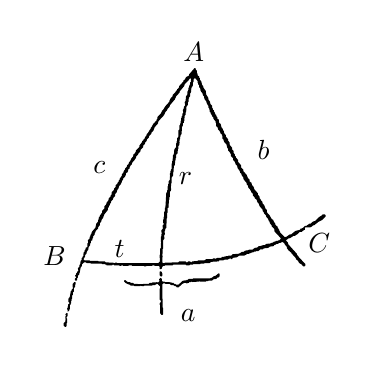
\begin{tikzpicture}[x=.00225in,y=-.00225in]
\path[use as bounding box] (0,0) rectangle (728,700);
\path[fill=black,even odd rule] (88,636) -- (87,636) -- (84,639) -- (85,641) -- (85,643) -- (84,644) -- (84,648) -- (85,650) -- (84,651) -- (84,655) -- (80,659) -- (80,664) -- (83,667) -- (85,667) -- (87,665) -- (87,659) -- (88,658) -- (88,649) -- (87,648) -- (87,645) -- (89,643) -- (89,637) -- cycle (106,567) -- (104,567) -- (100,572) -- (100,578) -- (101,579) -- (101,581) -- (98,584) -- (98,586) -- (96,588) -- (94,600) -- (91,604) -- (91,611) -- (93,613) -- (93,615) -- (90,617) -- (90,621) -- (89,622) -- (89,625) -- (88,626) -- (88,628) -- (89,629) -- (89,633) -- (90,633) -- (93,630) -- (93,628) -- (94,627) -- (94,619) -- (96,617) -- (96,615) -- (97,614) -- (97,609) -- (98,608) -- (98,605) -- (99,604) -- (99,597) -- (101,595) -- (101,590) -- (103,588) -- (103,581) -- (106,577) -- (106,573) -- (107,572) -- (107,568) -- cycle (428,549) -- (427,548) -- (425,548) -- (419,553) -- (415,554) -- (410,558) -- (408,558) -- (407,559) -- (369,559) -- (368,560) -- (359,560) -- (357,562) -- (355,562) -- (354,563) -- (346,564) -- (336,573) -- (331,573) -- (329,571) -- (326,571) -- (325,569) -- (321,569) -- (320,568) -- (317,568) -- (316,567) -- (306,567) -- (305,566) -- (301,566) -- (299,564) -- (299,560) -- (297,558) -- (296,558) -- (293,561) -- (294,565) -- (291,568) -- (289,568) -- (288,567) -- (286,568) -- (278,568) -- (277,569) -- (272,569) -- (270,571) -- (258,571) -- (257,572) -- (237,571) -- (235,569) -- (230,569) -- (228,567) -- (223,567) -- (218,563) -- (216,563) -- (215,564) -- (215,566) -- (218,569) -- (224,572) -- (226,572) -- (230,575) -- (237,575) -- (238,576) -- (251,576) -- (252,575) -- (254,576) -- (259,576) -- (260,575) -- (277,575) -- (278,574) -- (284,574) -- (286,572) -- (289,571) -- (295,577) -- (295,581) -- (294,582) -- (294,606) -- (297,609) -- (297,611) -- (294,615) -- (294,617) -- (295,618) -- (295,636) -- (298,640) -- (301,640) -- (302,639) -- (302,625) -- (301,624) -- (301,605) -- (300,604) -- (300,572) -- (302,570) -- (306,570) -- (307,571) -- (316,571) -- (320,574) -- (325,574) -- (328,576) -- (330,576) -- (332,578) -- (332,579) -- (336,579) -- (345,571) -- (349,569) -- (353,569) -- (354,570) -- (356,570) -- (357,569) -- (359,569) -- (360,567) -- (364,567) -- (365,566) -- (367,567) -- (382,566) -- (383,565) -- (385,566) -- (397,566) -- (398,565) -- (402,565) -- (403,564) -- (411,564) -- (414,561) -- (421,560) -- (421,559) -- (423,557) -- (425,557) -- (428,554) -- cycle (294,544) -- (294,552) -- (297,555) -- (298,555) -- (300,553) -- (300,548) -- (299,547) -- (299,545) -- (297,543) -- cycle (664,418) -- (662,416) -- (658,416) -- (655,419) -- (650,422) -- (641,431) -- (639,431) -- (635,433) -- (631,437) -- (628,437) -- (621,442) -- (618,442) -- (614,446) -- (610,448) -- (608,448) -- (608,449) -- (606,451) -- (597,453) -- (587,461) -- (584,461) -- (577,466) -- (573,467) -- (563,457) -- (563,455) -- (561,453) -- (561,451) -- (559,449) -- (559,447) -- (557,445) -- (557,443) -- (556,443) -- (552,439) -- (552,437) -- (549,433) -- (547,428) -- (546,428) -- (543,425) -- (539,418) -- (535,414) -- (533,410) -- (533,406) -- (530,403) -- (527,395) -- (524,392) -- (523,388) -- (520,385) -- (519,382) -- (517,380) -- (517,377) -- (513,372) -- (513,369) -- (505,360) -- (505,358) -- (503,354) -- (500,351) -- (499,346) -- (495,343) -- (495,340) -- (494,338) -- (491,335) -- (488,328) -- (481,320) -- (481,317) -- (476,312) -- (476,308) -- (475,306) -- (469,299) -- (469,295) -- (464,289) -- (464,287) -- (462,286) -- (462,283) -- (459,279) -- (459,275) -- (456,272) -- (456,268) -- (451,262) -- (450,260) -- (450,256) -- (447,252) -- (447,249) -- (442,243) -- (442,240) -- (438,235) -- (437,230) -- (435,228) -- (435,226) -- (432,222) -- (430,214) -- (429,214) -- (427,212) -- (427,210) -- (426,209) -- (426,205) -- (423,203) -- (423,200) -- (421,198) -- (420,194) -- (418,193) -- (418,191) -- (415,186) -- (415,184) -- (413,183) -- (413,181) -- (411,178) -- (411,174) -- (408,171) -- (407,169) -- (407,166) -- (403,160) -- (403,157) -- (398,149) -- (397,141) -- (392,134) -- (391,130) -- (389,128) -- (387,120) -- (384,116) -- (384,113) -- (382,111) -- (382,108) -- (381,108) -- (379,106) -- (379,104) -- (377,100) -- (377,96) -- (375,94) -- (374,90) -- (372,90) -- (360,104) -- (360,106) -- (358,108) -- (355,109) -- (352,112) -- (351,115) -- (347,118) -- (347,120) -- (338,130) -- (337,134) -- (334,137) -- (333,137) -- (333,139) -- (330,142) -- (330,143) -- (323,150) -- (323,153) -- (319,157) -- (316,163) -- (316,165) -- (307,175) -- (302,183) -- (300,185) -- (299,185) -- (299,187) -- (297,191) -- (290,198) -- (289,200) -- (289,203) -- (287,206) -- (287,208) -- (285,209) -- (283,211) -- (283,212) -- (279,215) -- (279,217) -- (277,219) -- (277,221) -- (274,224) -- (274,226) -- (272,228) -- (268,235) -- (265,238) -- (265,240) -- (261,245) -- (261,247) -- (258,250) -- (258,251) -- (255,253) -- (255,255) -- (249,263) -- (249,266) -- (241,274) -- (241,276) -- (239,280) -- (237,282) -- (236,282) -- (235,287) -- (230,293) -- (230,295) -- (225,302) -- (225,304) -- (223,306) -- (222,306) -- (221,310) -- (217,314) -- (217,316) -- (214,320) -- (214,322) -- (210,327) -- (210,330) -- (205,337) -- (205,339) -- (203,341) -- (203,343) -- (200,346) -- (200,348) -- (196,351) -- (196,355) -- (193,358) -- (192,362) -- (188,366) -- (187,368) -- (187,372) -- (185,374) -- (185,376) -- (181,380) -- (180,385) -- (176,390) -- (175,394) -- (171,398) -- (171,403) -- (167,407) -- (166,409) -- (166,412) -- (161,419) -- (161,421) -- (159,422) -- (158,428) -- (157,429) -- (157,432) -- (153,437) -- (151,446) -- (144,454) -- (142,458) -- (142,460) -- (140,462) -- (140,465) -- (138,467) -- (138,470) -- (134,474) -- (135,479) -- (133,481) -- (133,489) -- (129,491) -- (129,494) -- (127,496) -- (127,499) -- (125,501) -- (125,503) -- (124,504) -- (124,509) -- (122,511) -- (122,513) -- (120,514) -- (120,518) -- (118,520) -- (117,528) -- (115,529) -- (115,533) -- (112,536) -- (113,542) -- (111,544) -- (110,544) -- (110,546) -- (108,548) -- (108,550) -- (106,552) -- (106,554) -- (108,556) -- (108,557) -- (105,560) -- (105,562) -- (107,564) -- (109,564) -- (110,563) -- (110,559) -- (112,557) -- (112,553) -- (115,550) -- (115,547) -- (116,546) -- (118,535) -- (121,531) -- (121,528) -- (126,523) -- (130,523) -- (132,525) -- (140,525) -- (141,526) -- (165,526) -- (166,527) -- (172,527) -- (173,528) -- (175,528) -- (176,530) -- (188,530) -- (190,528) -- (191,528) -- (193,530) -- (204,530) -- (205,531) -- (208,531) -- (209,530) -- (212,530) -- (213,531) -- (224,531) -- (225,530) -- (232,530) -- (233,531) -- (259,531) -- (260,532) -- (264,532) -- (265,531) -- (277,531) -- (278,530) -- (282,530) -- (283,531) -- (292,531) -- (294,533) -- (294,537) -- (295,538) -- (297,538) -- (299,537) -- (299,535) -- (302,531) -- (305,531) -- (306,530) -- (323,530) -- (325,528) -- (352,528) -- (354,530) -- (360,530) -- (362,528) -- (368,528) -- (369,527) -- (384,527) -- (385,526) -- (393,526) -- (394,525) -- (405,525) -- (409,522) -- (426,521) -- (427,519) -- (435,519) -- (439,517) -- (446,517) -- (447,516) -- (449,516) -- (451,514) -- (452,514) -- (453,516) -- (456,516) -- (456,515) -- (458,513) -- (466,512) -- (472,508) -- (483,508) -- (487,506) -- (489,504) -- (493,504) -- (500,501) -- (503,501) -- (505,499) -- (508,499) -- (509,498) -- (514,498) -- (519,494) -- (524,494) -- (526,492) -- (536,491) -- (540,488) -- (548,487) -- (550,484) -- (552,484) -- (555,482) -- (558,482) -- (560,480) -- (563,480) -- (567,478) -- (569,478) -- (573,482) -- (573,483) -- (578,489) -- (578,492) -- (580,494) -- (580,495) -- (588,502) -- (588,503) -- (598,514) -- (598,516) -- (603,520) -- (604,523) -- (607,526) -- (610,527) -- (614,532) -- (617,532) -- (619,530) -- (619,527) -- (604,511) -- (604,510) -- (601,507) -- (600,504) -- (581,483) -- (580,479) -- (576,475) -- (576,474) -- (581,470) -- (585,469) -- (593,464) -- (596,464) -- (598,462) -- (602,460) -- (607,455) -- (611,455) -- (616,451) -- (618,451) -- (618,446) -- (619,445) -- (630,445) -- (634,443) -- (636,441) -- (638,441) -- (648,433) -- (656,429) -- (664,421) -- cycle (363,113) -- (365,115) -- (364,116) -- (364,121) -- (362,122) -- (362,126) -- (360,130) -- (360,133) -- (358,135) -- (358,139) -- (356,143) -- (356,149) -- (353,153) -- (352,163) -- (350,166) -- (351,173) -- (348,177) -- (348,180) -- (346,184) -- (347,190) -- (345,192) -- (345,196) -- (343,198) -- (343,201) -- (342,202) -- (342,207) -- (341,208) -- (341,213) -- (340,214) -- (340,216) -- (338,218) -- (338,227) -- (336,229) -- (336,243) -- (333,247) -- (333,253) -- (332,254) -- (332,257) -- (331,258) -- (331,266) -- (327,271) -- (326,282) -- (324,284) -- (323,297) -- (322,298) -- (322,302) -- (321,303) -- (321,315) -- (319,317) -- (319,319) -- (318,320) -- (318,324) -- (317,325) -- (317,329) -- (318,330) -- (317,332) -- (317,339) -- (314,343) -- (314,348) -- (313,349) -- (313,353) -- (312,354) -- (312,362) -- (311,363) -- (311,366) -- (309,368) -- (307,401) -- (306,402) -- (306,409) -- (304,411) -- (304,421) -- (303,422) -- (303,427) -- (302,428) -- (302,435) -- (303,436) -- (303,439) -- (301,441) -- (301,445) -- (302,447) -- (298,452) -- (298,456) -- (299,457) -- (299,459) -- (298,460) -- (298,465) -- (297,466) -- (297,477) -- (298,479) -- (297,480) -- (297,491) -- (295,493) -- (295,506) -- (294,507) -- (295,521) -- (291,525) -- (200,525) -- (199,524) -- (195,524) -- (194,525) -- (192,525) -- (191,524) -- (181,524) -- (180,523) -- (174,523) -- (172,521) -- (158,521) -- (157,520) -- (139,520) -- (138,519) -- (127,519) -- (125,517) -- (125,515) -- (128,510) -- (128,507) -- (131,504) -- (132,499) -- (135,495) -- (136,489) -- (139,485) -- (139,482) -- (141,479) -- (141,476) -- (143,474) -- (144,474) -- (144,471) -- (146,468) -- (146,465) -- (149,462) -- (149,460) -- (152,453) -- (157,448) -- (157,445) -- (161,440) -- (161,436) -- (164,432) -- (165,428) -- (168,424) -- (171,416) -- (179,406) -- (179,402) -- (181,400) -- (181,397) -- (183,396) -- (183,394) -- (186,389) -- (186,387) -- (190,383) -- (191,379) -- (195,375) -- (195,371) -- (198,368) -- (200,361) -- (202,359) -- (204,353) -- (207,350) -- (210,344) -- (210,342) -- (213,338) -- (213,336) -- (216,333) -- (217,333) -- (217,331) -- (219,328) -- (219,325) -- (221,323) -- (222,323) -- (224,319) -- (224,316) -- (227,314) -- (227,312) -- (229,308) -- (232,305) -- (233,301) -- (239,294) -- (242,289) -- (242,287) -- (246,283) -- (247,280) -- (251,276) -- (252,272) -- (257,267) -- (258,262) -- (260,260) -- (261,260) -- (262,256) -- (265,253) -- (266,249) -- (270,245) -- (271,241) -- (276,236) -- (276,234) -- (280,230) -- (283,222) -- (291,213) -- (291,210) -- (292,208) -- (304,195) -- (307,188) -- (310,185) -- (312,181) -- (316,177) -- (317,173) -- (328,160) -- (331,153) -- (336,148) -- (336,147) -- (339,144) -- (339,142) -- (349,130) -- (350,126) -- (360,116) -- (360,115) -- (362,113) -- cycle (373,112) -- (379,119) -- (379,123) -- (380,124) -- (380,126) -- (382,128) -- (382,132) -- (385,136) -- (385,139) -- (387,143) -- (389,145) -- (391,151) -- (393,153) -- (394,159) -- (398,164) -- (399,168) -- (401,172) -- (403,174) -- (403,178) -- (405,181) -- (406,188) -- (408,189) -- (408,191) -- (411,196) -- (411,198) -- (412,198) -- (414,200) -- (414,203) -- (419,209) -- (419,212) -- (420,213) -- (420,219) -- (424,223) -- (424,226) -- (429,232) -- (430,236) -- (431,236) -- (433,238) -- (433,240) -- (434,241) -- (434,247) -- (437,250) -- (437,252) -- (439,256) -- (443,260) -- (445,268) -- (447,270) -- (447,274) -- (450,277) -- (453,282) -- (453,286) -- (458,291) -- (458,295) -- (461,298) -- (463,302) -- (463,304) -- (467,308) -- (468,313) -- (473,320) -- (474,324) -- (476,325) -- (477,329) -- (481,334) -- (481,337) -- (482,339) -- (488,346) -- (488,349) -- (491,352) -- (492,357) -- (496,361) -- (496,362) -- (498,364) -- (498,366) -- (502,370) -- (502,374) -- (506,378) -- (506,380) -- (511,384) -- (511,386) -- (513,390) -- (515,392) -- (517,398) -- (524,406) -- (524,409) -- (526,411) -- (527,414) -- (531,418) -- (532,422) -- (535,425) -- (537,429) -- (537,431) -- (539,432) -- (540,436) -- (544,441) -- (544,443) -- (549,448) -- (550,450) -- (550,454) -- (564,469) -- (564,471) -- (561,474) -- (559,474) -- (558,475) -- (554,475) -- (552,477) -- (549,477) -- (547,479) -- (543,480) -- (542,481) -- (532,482) -- (528,485) -- (524,485) -- (523,486) -- (520,486) -- (519,487) -- (515,487) -- (512,490) -- (506,491) -- (501,495) -- (493,495) -- (492,496) -- (485,497) -- (481,500) -- (477,500) -- (473,503) -- (471,503) -- (470,504) -- (457,505) -- (454,508) -- (448,508) -- (447,509) -- (443,509) -- (442,510) -- (439,510) -- (438,511) -- (433,511) -- (432,513) -- (423,513) -- (419,515) -- (415,514) -- (411,516) -- (398,516) -- (394,519) -- (380,519) -- (379,520) -- (367,521) -- (365,523) -- (364,523) -- (362,521) -- (358,521) -- (356,523) -- (354,523) -- (352,521) -- (338,521) -- (336,523) -- (322,523) -- (321,524) -- (306,524) -- (305,525) -- (302,525) -- (300,523) -- (300,512) -- (301,511) -- (301,509) -- (300,508) -- (300,504) -- (301,503) -- (301,493) -- (302,492) -- (302,474) -- (305,470) -- (305,467) -- (304,466) -- (304,464) -- (306,460) -- (305,454) -- (306,453) -- (307,448) -- (309,446) -- (310,425) -- (311,424) -- (311,413) -- (312,412) -- (312,402) -- (314,401) -- (314,392) -- (315,391) -- (315,384) -- (316,383) -- (316,378) -- (317,377) -- (317,366) -- (319,364) -- (319,362) -- (320,361) -- (320,359) -- (319,358) -- (319,354) -- (320,353) -- (320,347) -- (321,346) -- (321,334) -- (324,330) -- (324,323) -- (325,322) -- (326,308) -- (328,306) -- (329,296) -- (330,295) -- (330,291) -- (331,290) -- (331,283) -- (334,280) -- (334,275) -- (335,274) -- (335,271) -- (336,270) -- (336,264) -- (338,262) -- (338,258) -- (339,257) -- (338,253) -- (339,252) -- (339,249) -- (340,248) -- (340,243) -- (341,242) -- (341,239) -- (343,237) -- (344,222) -- (346,218) -- (346,213) -- (348,212) -- (348,209) -- (349,208) -- (350,196) -- (352,194) -- (352,189) -- (353,188) -- (353,185) -- (354,184) -- (354,176) -- (357,172) -- (357,167) -- (359,164) -- (359,158) -- (360,157) -- (360,155) -- (362,153) -- (362,147) -- (364,144) -- (365,134) -- (367,132) -- (367,130) -- (368,129) -- (368,123) -- (370,120) -- (370,115) -- cycle;
\node[inner sep=0pt,font=\normalsize] at (370,55) {$A$};
\node[inner sep=0pt,font=\normalsize] at (60,510) {$B$};
\node[inner sep=0pt,font=\normalsize] at (650,481) {$C$};
\node[inner sep=0pt,font=\normalsize] at (358,641) {$a$};
\node[inner sep=0pt,font=\normalsize] at (526,273) {$b$};
\node[inner sep=0pt,font=\normalsize] at (160,312) {$c$};
\node[inner sep=0pt,font=\normalsize] at (352,336) {$r$};
\node[inner sep=0pt,font=\normalsize] at (205,493) {$t$};
\end{tikzpicture}
\end{center}
\noindent\hspace*{1.2em}[Ferner ist] allgemein
